Pour pouvoir transmettre les messages depuis l'utilisateur vers le téléphone portable, nous avons
choisi de mettre en place un site web à l'allure d'un gestionnaire de conversation. 
blablabla

Le fonctionnement de ce projet repose grandement sur la partie qui suit.



%%%%%%%%%%%%%%%%%%%%%%%%%%%%%%%%%%%%%%%%%%%%%%%%%%%%%%%%%%%%%%%%%%%%%%%%%%%%%%%%%%%%%%%%%%%%%%%%%%%%
\subsection{Play Framework 2.0}
%%%%%%%%%%%%%%%%%%%%%%%%%%%%%%%%%%%%%%%%%%%%%%%%%%%%%%%%%%%%%%%%%%%%%%%%%%%%%%%%%%%%%%%%%%%%%%%%%%%%

\subsubsection{Primefaces vs Play Framework}

Pour créer notre webservice, nous souhaitions utiliser des technologies récentes. Nous nous sommes
alors confrontés à deux choix complètement opposés. Premièrement, utilisé le jeune Play Framework 
qui est un framework d'application web RESTFul. Le deuxième candidat, Primefaces, est un framework
basé sur les JSF. Il contient une bibliothèque graphique très riche.

Notre choix s'est porté sur Play dont l'approche original nous à attirer. Play Framework est basé sur
les langages Java et Scala et permet le développement sur ces deux langages. C'est un framework RESTFul
ce qui implique que le serveur ne gère pas d'état pour les clients.


%%%%%%%%%%%%%%%%%%%%%%%%%%%%%%%%%%%%%%%%%%%%%%%%%%%%%%%%%%%%%%%%%%%%%%%%%%%%%%%%%%%%%%%%%%%%%%%%%%%%
\subsection{Authentification avec OAuth 2.0}
\label{Authentification avec OAuth 2.0}
%%%%%%%%%%%%%%%%%%%%%%%%%%%%%%%%%%%%%%%%%%%%%%%%%%%%%%%%%%%%%%%%%%%%%%%%%%%%%%%%%%%%%%%%%%%%%%%%%%%%

L'authentification des utilisateurs est un point sensible lors du développement d'un service car il
implique souvent le stockage des mots de passes et donc de sécuriser l'application, veiller à corriger
les failles de sécurité, ... 

%%%%%%%%%%%%%%%%%%%%%%%%%%%%%%%%%%%%%%%%%%%%%%%%%%%%%%%%%%%%%%%%%%%%%%%%%%%%%%%%%%%%%%%%%%%%%%%%%%%%

\subsubsection{OAuth 2.0}

\textit{OAuth}\footnote{Site web : \href{http://oauth.net/}{http://oauth.net/}} est un protocole standard et libre d'accès aux données.
Il permet l'authentification à une API en demandant à l'utilisateur les données qu'il souhaite partager.
La gestion des utilisateurs se fait ensuite grâce à un "jeton", appelé "token" par la suite, unique délivré par le service tiers.

Beaucoup de services internet populaire implémentent ce système ce qui permet de aux utilisateurs de se connecter à un service en utilisant un de leurs comptes déjà existant.
C'est le cas par exemple de Deezer ou de Stack Overflow qui proposent de s'identifier avec un compte Google, Facebook, Twitter, Windows Live ou autre.
Ce protocole facilite donc la connexion pour le service qui l'utilise et les utilisateurs qui n'ont pas 
à créer un nouveau compte sur chaque nouveau site web par exemple.
\\


Nous avons alors décider d'utiliser OAuth 2.0 pour deux raisons importantes.
La première concerne la gestion des utilisateurs sur notre service web qui n'aura pas lieu d'être, ce qui facilite le développement en laissant Google s'occuper de la sécurité, et le fait que nous voulions proposer une solution sans enregistrement des informations des utilisateurs.
La seconde raison concerne l'accès aux données et aux services du compte Google, qui nous permettra l'accès aux contacts et à GTalk.
OAuth s'est donc avéré comme la solution idéale pour notre projet.

%%%%%%%%%%%%%%%%%%%%%%%%%%%%%%%%%%%%%%%%%%%%%%%%%%%%%%%%%%%%%%%%%%%%%%%%%%%%%%%%%%%%%%%%%%%%%%%%%%%%

\subsubsection{Fonctionnement}

\begin{figure}[!h]
	\center
	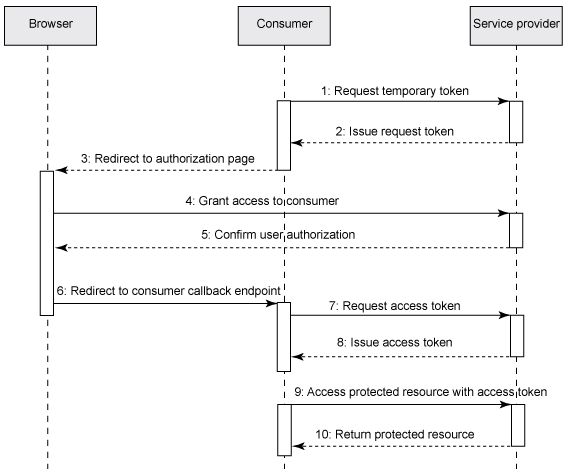
\includegraphics[width=0.8\textwidth]{img/OAuth_fonctionnement.png}
	\caption{OAuth : fonctionnement}
	Source : \href{http://www.ibm.com/developerworks/web/library/wa-oauthsupport/ThreeLeggedOAuthDance.gif}{http://www.ibm.com}
	\label{OAuth_fonctionnement}
\end{figure}

L'authentification se déroule en plusieurs étapes présentées dans le schéma \ref{OAuth_fonctionnement}.
\\


\begin{figure}[!h]
	\center
	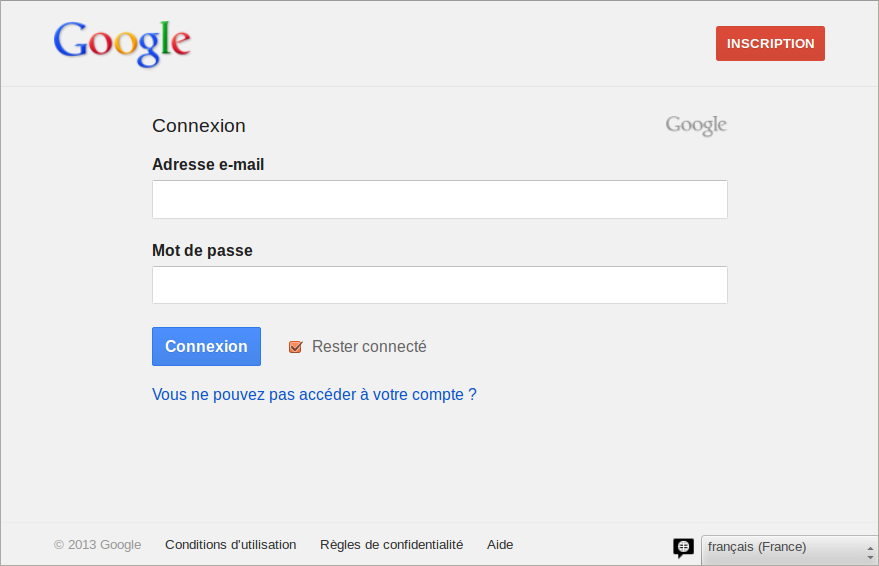
\includegraphics[width=0.6\textwidth]{img/OAuth_authentificationGoogle.png}
	\caption{OAuth : authentification sur Google}
	\label{OAuth_authentificationGoogle}
\end{figure}

Premièrement l'utilisateur doit s'authentifier sur la plateforme de l'API proposant le service OAuth.
Dans notre cas il s'agit de Google, comme le montre la capture \ref{OAuth_authentificationGoogle}.
\\


\begin{figure}[!h]
	\center
	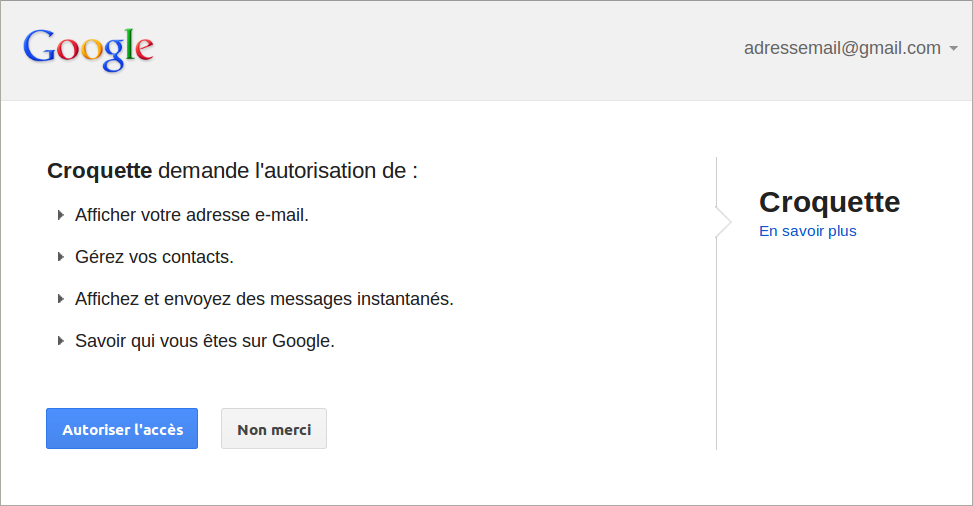
\includegraphics[width=0.6\textwidth]{img/OAuth_demandeAutorisations.png}
	\caption{OAuth : demande d'autorisation}
	\label{OAuth_demandeAutorisations}
\end{figure}

Ensuite l'utilisateur est redirigé vers la page des autorisations où il doit accepter les demandes de l'application.
Dans notre cas il s'agit de récupérer les contacts et d'utiliser le compte GTalk de l'utilisateur, comme le montre la capture d'écran \ref{OAuth_demandeAutorisations}.

Si l'authentification réussi alors l'application se voit offrir un token.
Elle doit alors l'échanger avec les serveurs de Google dans le but d'obtenir un token d'accès.
Si tout se déroule correctement elle obtient le token d'accès.
\\


Lors de chaque requête pour récupérer des informations sur l'utilisateur, le webservice devra alors
joindre son token d'accès à la requête pour avoir une réponse. De cette manière, nous pouvons récupérer
des informations de l'utilisateur sans utiliser son mot de passe et son identifiant. Nous déléguons donc
la sécurisation du mot de passe à Google.

Nous avons choisi d'utiliser l'authentification avec la plateforme Google car nous pouvions ainsi 
successivement, s'authentifier sur GTalk et récupérer les contacts de l'utilisateur.



%%%%%%%%%%%%%%%%%%%%%%%%%%%%%%%%%%%%%%%%%%%%%%%%%%%%%%%%%%%%%%%%%%%%%%%%%%%%%%%%%%%%%%%%%%%%%%%%%%%%
%%%%%%%%%%%%%%%%%%%%%%%%%%%%%%%%%%%%%%%%%%%%%%%%%%%%%%%%%%%%%%%%%%%%%%%%%%%%%%%%%%%%%%%%%%%%%%%%%%%%
%%%%%%%%%%%%%%%%%%%%%%%%%%%%%%%%%%%%%%%%%%%%%%%%%%%%%%%%%%%%%%%%%%%%%%%%%%%%%%%%%%%%%%%%%%%%%%%%%%%%

\subsection{Gestion des contacts}

La gestion des contacts de l'utilisateur est un point important de notre projet.
De plus notre cahier des charges spécifie leurs gestion simple et transparente.

%%%%%%%%%%%%%%%%%%%%%%%%%%%%%%%%%%%%%%%%%%%%%%%%%%%%%%%%%%%%%%%%%%%%%%%%%%%%%%%%%%%%%%%%%%%%%%%%%%%%

\subsubsection{Téléchargement des contacts Google}
\label{Téléchargement des contacts Google}

Par défaut sous Androïd les contacts du téléphone sont dupliqués sur le serveur Google grâce au compte associés au smartphone, ce qui permet d'avoir une synchronisation sur tous les services Google dont Gmail.

Étant connecté sur notre site internet via son compte Google, notre application web va ainsi pouvoir récupérer la liste des contacts de l'utilisateur grâce au token délivré par Google lors de l'authentification.

%%%%%%%%%%%%%%%%%%%%%%%%%%%%%%%%%%%%%%%%%%%%%%%%%%%%%%%%%%%%%%%%%%%%%%%%%%%%%%%%%%%%%%%%%%%%%%%%%%%%

\subsubsection{Tri et Formatage}

Le carnet de contacts de l'utilisateur peut contenir de nombreux types de numéros : téléphone mobiles, téléphone fixes, numéros étrangers, numéros surtaxés, ...
Nous avons donc filtré la liste des contacts aux numéros de mobiles, c'est-à-dire ceux commençant par "0" ou "+33" suivi de 9 chiffres.

Cela permet de ne pas surcharger la liste des contacts avec de nombreux numéros à qui l'on envoie jamais de SMS.
De plus c'est un aspect sécuritaire car l'utilisateur ne pourra pas envoyer des SMS surtaxés depuis le site web.
Un autre point important et le formatage des contacts. En effet nous allons systématiquement récupérés les contacts
et les modifiés afin de les rendre uniformes. Nous voulions avoir pour chaque contact, un nom et un prénom
dont les premières lettres uniquement soit en majuscules. De plus, nous souhaitions récupéré plusieurs fois
un contact qui possède plusieurs numéros de téléphones.

%%%%%%%%%%%%%%%%%%%%%%%%%%%%%%%%%%%%%%%%%%%%%%%%%%%%%%%%%%%%%%%%%%%%%%%%%%%%%%%%%%%%%%%%%%%%%%%%%%%%

\subsubsection{Google Guava}

Une fois la liste des contacts téléchargés il est nécessaire de la stocker sur le serveur pour ne pas avoir à la télécharger après chaque rafraichissement de page.
Il existe plusieurs méthodes permettant le stockage.

Une \textit{base de données} permet de stocker efficacement des données.
Nous avons voulu proposer aux utilisateurs une solution "sûre" dans laquelle aucune donnée ne sera enregistrées sur le serveur, ce qui implique que l'on n'utilisera pas cette méthode.

La \textit{session} est une courte période pendant laquelle le serveur web communique avec le client (l'utilisateur).
Durant cette période une quantité de mémoire est allouée au client pour y stocker différentes informations, que l'on appelle "variable de session".
Dans Play la notion de "session" est quasiment inexistante en raison de sa nature "RESTful", c'est-à-dire qui ne conserve pas de données liées aux clients durant la session.

Pour palier ce manque Play propose l'utilisation de \textit{caches}, qui est une zone mémoire à association clé-valeur commune à toutes les utilisateurs mais avec une durée de vie limitée.
Lorsque le délai est écoulé les données sont effacées automatiquement.
Le problème de cette solution sont les nombreux tests à effectuer pour vérifier que les données sont toujours présentes et effectuer la mise à jour à chaque fois que le cache est vidé.

Nous avons utilisé la classe \lstinline{CacheBuilder} de la bibliothèque Java \textit{Guava} proposé par Google.
Cette classe agit globalement comme un cache (association clé-valeur, durée de vie limitée) tout en proposant de nombreuses fonctionnalités.
Il est notamment possible de définir une fonction qui sera exécutée lors de chaque "mise à jour" du cache, la durée de vie du cache, le nombre maximum de données, ...



%%%%%%%%%%%%%%%%%%%%%%%%%%%%%%%%%%%%%%%%%%%%%%%%%%%%%%%%%%%%%%%%%%%%%%%%%%%%%%%%%%%%%%%%%%%%%%%%%%%%
\subsection{Communication entre le serveur web et le navigateur du client}
%%%%%%%%%%%%%%%%%%%%%%%%%%%%%%%%%%%%%%%%%%%%%%%%%%%%%%%%%%%%%%%%%%%%%%%%%%%%%%%%%%%%%%%%%%%%%%%%%%%%

L'un des points clés du framework Play est sa capacité à gérer les websockets. Il fait en effet partis des rares
frameworks offrant cette fonctionnalité relativement récente. Le protocole websocket vise à établir 
une communication bidirectionnelle et full duplex entre un navigateur web et un serveur. Cela signifie
qu'un lien de communication s'établit entre les deux entités et permet la communication simultanée
dans les deux sens. 

%%%%%%%%%%%%%%%%%%%%%%%%%%%%%%%%%%%%%%%%%%%%%%%%%%%%%%%%%%%%%%%%%%%%%%%%%%%%%%%%%%%%%%%%%%%%%%%%%%%%

\subsubsection{Websocket}

Pour ce projet, les fonctionnalités des websockets étaient une véritable aubaine car elles nous permettaient
lors d'un changement d'état coté serveur d'avertir le client web. Dans notre cas, le serveur souhaite avertir
le client lors de la réception d'un SMS et le client souhaite avertir le serveur lors de l'envoi d'un message
XMPP. Les websockets sont donc adaptés à cette situation. Elles sont la clé de voute de ce projet car elles 
s'occupent des communications entre le client et le serveur.

Une fois que l'utilisateur s'est authentifié, plus aucun rechargement de pages ne sera fait.
Tout est géré 
dynamiquement via les websockets. 

La prise en charge du coté serveur se fait avec le framework Play qui gère nativement les websockets. Coté client,
c'est le navigateur qui à l'aide du langage JavaScript va gérer les websockets. Celles-ci sont en cours de standardisation
du coté du W3C et les différents navigateur les implémentent donc chacun à leurs façons. 

En ce qui nous concerne, nous avons choisi de ne travailler que sur les navigateurs Mozilla Firefox et Google Chrome.
Ce projet est donc inutilisable aujourd'hui sur d'autres navigateurs.

Pour pouvoir communiquer les SMS et message XMPP, nous avons choisi d'utiliser le format JSON qui est le format de
donnée naturel pour les applications JavaScript. De plus, puisque nous utilisons ce format pour faire transiter les
données entre les applications mobiles et le serveur, c'était pour nous très pratique de ne pas avoir à modifier
les données lors des différents échanges.

%%%%%%%%%%%%%%%%%%%%%%%%%%%%%%%%%%%%%%%%%%%%%%%%%%%%%%%%%%%%%%%%%%%%%%%%%%%%%%%%%%%%%%%%%%%%%%%%%%%%

\subsubsection{Notifications}

Les messages XMPP et SMS ne sont pas les seuls à transiter sur les websockets. En effet nous avons 
implémenter de la même manière un système de notification de nouveau message. Le système est simple,
lors de la réception d'un nouveau message, si l'utilisateur ne dialogue pas au même moment avec l'auteur
du nouveau message, une notification va s'afficher. Comme le montre l'image \ref{siteWeb_notifications}, le contact
qui a envoyé le message verra un compteur apparaitre à coté de son nom. Cela permet simplement d'avertir
l'utilisateur courant du nombre de message non lus envoyés par un de ses contacts.
\begin{figure}[!h]
	\center
	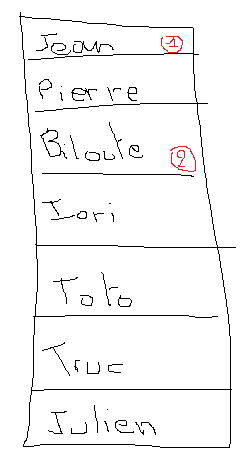
\includegraphics[width=0.2\textwidth]{img/siteWeb_notifications.png}
	\caption{Site web : notifications}
	\label{siteWeb_notifications}
\end{figure}

%%%%%%%%%%%%%%%%%%%%%%%%%%%%%%%%%%%%%%%%%%%%%%%%%%%%%%%%%%%%%%%%%%%%%%%%%%%%%%%%%%%%%%%%%%%%%%%%%%%%

\subsection{Design du site}

Le design du site est l'un des thèmes que nous avons travaillé pour cette partie la du projet.

Nous souhaitions initialement avoir une interface simple, sans fioritures car cela nous semblait comme
secondaire. Nous avons donc utilisé deux frameworks pour nous faciliter la tache et accélérer la mise
en place du design.

Nous avons donc tout d'abord choisi "Twitter Bootstrap" puis nous l'avons couplé au framework "jQuery
Layout".

%%%%%%%%%%%%%%%%%%%%%%%%%%%%%%%%%%%%%%%%%%%%%%%%%%%%%%%%%%%%%%%%%%%%%%%%%%%%%%%%%%%%%%%%%%%%%%%%%%%%

\subsubsection{Twitter Bootstrap}

\textit{Twitter Bootstrap}\footnote{Site web : \href{http://twitter.github.com/bootstrap/}{http://twitter.github.com/bootstrap/}} est un framework web utilisé pour le développement front end.
C'est un outil écrit en JavaScript et CSS qui permet de réaliser facilement des interfaces élégantes néanmoins simples. 

Il nous a été utile principalement pour pouvoir concevoir l'affichage des zones d'entrée de textes ou 
encore pour organiser l'affichage des contacts proprement.

%%%%%%%%%%%%%%%%%%%%%%%%%%%%%%%%%%%%%%%%%%%%%%%%%%%%%%%%%%%%%%%%%%%%%%%%%%%%%%%%%%%%%%%%%%%%%%%%%%%%

\subsubsection{jQuery Layout}

\textit{jQuery Layout}\footnote{Site web : \href{http://layout.jquery-dev.net/}{http://layout.jquery-dev.net/}} est aussi un framework web qui, contrairement à Twitter Bootstrap, permet d'organiser les sites en plusieurs interfaces distinctes. 
L'utilité de JQuery Layout réside dans sa possibilité à fractionner un espace en plusieurs fenêtres.
Cela permet de retrouver l'ergonomie et le coté simple et ordonné des logiciels. 

Ce framework très riche nous a donc été très profitable pour pouvoir obtenir une bonne ergonomie sans avoir
à trop passer du temps sur cette partie.
Le schéma \ref{siteWeb_jQueryLayout} représente l'agencement général de notre site web grâce à ce framework.

\begin{figure}[!h]
	\center
	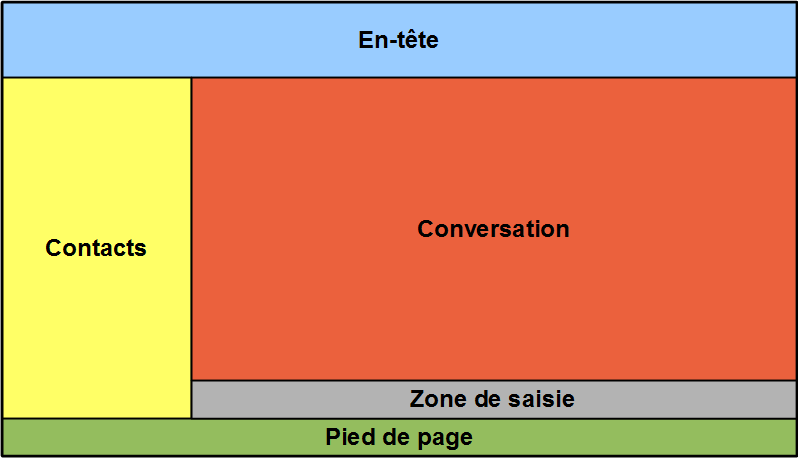
\includegraphics[width=0.6\textwidth]{img/siteWeb_jQueryLayout.png}
	\caption{jQuery Layout : structure du site web}
	\label{siteWeb_jQueryLayout}
\end{figure}
